% Metódy inžinierskej práce

\documentclass[10pt,twoside,slovak,a4paper]{article}

\usepackage[slovak]{babel}
%\usepackage[T1]{fontenc}
\usepackage[IL2]{fontenc} % lepšia sadzba písmena Ľ než v T1
\usepackage[utf8]{inputenc}
\usepackage{graphicx}
\usepackage[thinlines]{easytable}
\usepackage{url} % príkaz \url na formátovanie URL
\usepackage{hyperref} % odkazy v texte budú aktívne (pri niektorých triedach dokumentov spôsobuje posun textu)
\graphicspath{ {./images/} }
\usepackage{cite}
\usepackage{pdfpages}
%\usepackage{times}

\pagestyle{plain}

\title{Aplikovanie hier v procese vzdelávania
%\thanks{Semestrálny projekt v predmete Metódy inžinierskej práce, ak. rok 2022/23, vedenie: Igor Stupavský}
} % meno a priezvisko vyučujúceho na cvičeniach

\author{Patrik Drdák\\[2pt]
	{\small Slovenská technická univerzita v Bratislave}\\
	{\small Fakulta informatiky a informačných technológií}\\
	{\small \texttt{xdrdak@stuba.sk}}
	}

\date{\small 19. október 2022} % upravte


\begin{document}

\maketitle

\begin{abstract}
Tento príspevok rozoberá aplikovanie hier
ako edukačnej pomôcky na príjem informácií ale taktiež interagovanie s nimi,
čo vo výsledku by malo mať pozitívny vplyv na efektivitu učenia sa a samotné
učenie. Použitie týchto hier by malo mať takisto pozitívny vplyv na komunikáciu medzi študentom a pedagógom ako aj medzi študentmi navzájom. Súčasťou príspevku je taktiež zameranie sa na efektivitu používania vzdelávacích hier, to znamená na dosiahnuté výsledky v porovnaní s tými bez použitia týchto hier.

\end{abstract}



\section{Úvod}

Hra nie je iba pre deti a je známe, že najviac informácií si vieme zapamätať, keď máme z edukácie zážitok a vytvoria v nás pozitívnu emočnú stopu. A o tom využitie herných prvkov v nehernom prostredí práve je. Napriek preukázaným výhodám Serious Games v porovnaní s tradičným e-learningom, využívanie učenia založeného na hrách
v bežnom vzdelávaní je stále veľmi nízke. Zvýšená absorpcia
vyžaduje uľahčenie nasadenia vhodných hier ako typu aktivity
v existujúcich e-learningových platformách. Hlavné ciele gamifikácie sú zlepšenie určitých schopností, zapojenie študentov, optimalizovanie učenie, podporovanie zmeny správania a socializovanie sa. Stimulovaní efektmi, ktoré môžu herné prvky vyvolať, mnohí výskumníci skúmali vplyv gamifikácia vo vzdelávacom kontexte, pričom dosiahli priaznivé výsledky, ako je zvýšenie angažovanosti, pozornosti, vedomostí a spolupráce. Napriek tomu niektoré štúdie ukázali neisté alebo škodlivé výsledky gamifikácie. Zistili, že hodnotenie ovplyvňuje ženy rôznymi spôsobmi a môže viesť k neočakávanému opačnému vplyvu.

\section{Čo je to gamifikácia}
Asi najlepšie vieme gamifikáciu pochopiť na vernostných programoch rôznych obchodných reťazcov, kde zákazníci po každom nákupe obdržia určitý počet bodov na svoj účet.\cite{jakub-Framework} Po nazbieraní určitého počtu bodov zákazník získa zľavu na ďalší nákup alebo obdrží darček. To motivuje zákazníka k opätovným nákupov a tým sa zvyšuje zisk firmy. Podobne to funguje aj vo vzdelávaní, kde žiaci za rôzne úlohy získavajú určitý počet bodov, hodnotenie, a sú motivovaný k opätovnému riešenie ďalších úloh.  Gamifikácia nezahŕňa hry. Je to jednoducho absorbovanie zábavných prvkov v hre ,teda to, čo nazývame herná mechanika  alebo techniky dizajnu hier, do aplikácií v reálnom svete.



\section{Gamifikácia vs. hry} 
Učenie založené na hrách robí hry súčasťou vzdelávacieho procesu.
Je to metóda, pri ktorej sa študenti učia špecifické zručnosti alebo vedomosti z hrania hry.
Tento typ učenia preberá obsah učenia a premieňa ho na hru, ktorú môžu študenti hrať.
Na druhej strane gamifikácia využíva herné prvky iba v nehernom kontexte, aby sa zlepšilo porozumenie obsahu a podporilo sa lepšie uchovávanie informácií.
Hlavným cieľom je stále zlepšovať angažovanosť študentov a nemusí znamenať, že sa študenti naučia niečo nové. Hry majú úžasnú schopnosť udržať ľudí zapojených na dlhú dobu, budovať vzťahy a dôveru medzi ľuďmi a rozvíjať ich tvorivý potenciál.


\section{Gamifikácia vo vzdelaní} 

Existuje množstvo stratégií gamifikácie, ktoré môžete začleniť do svojho vzdelávacieho prostredia.
Najpopulárnejšie sú\cite{buljan}: 
\subsection{Bodové systémy}
    \begin{itemize}
    \item Prideľovanie bodov za splnenie rôznych úloh môže povzbudiť    jednotlivcov k tvrdej práci.
    \end{itemize}

\subsection{Odznaky}
    
    \begin{itemize}
    \item  Odznaky sú fantastickým spôsobom, ako oceniť a odmeniť ľudí za ich úsilie.Odznak je ocenenie udelené vo forme virtuálneho predmetu alebo pripnutého obrázka na vašom profile
    \end{itemize}
 
\subsection{Rebríčky} 

    \begin{itemize}
    \item Rebríčky sú skvelé na vytváranie konkurencie medzi študentmi, pretože budú chcieť vidieť svoje meno na vrchole a v dôsledku toho budú tvrdšie pracovať.
    \end{itemize}
Ľudia si myslia, že pri gamifikácii ide iba o pridávanie rôznych bodov a odznakov.
Aj keď sú odznaky a rebríčky súčasťou gamifikácie, nevystihujú však jej základnú podstatu.\cite{chou}Gamifikácia totiž využíva hernú mechaniku a techniky na zapojenie a motiváciu ľudí, takže nejde len o bezvýznamné rozdávanie odznakov, bodov a vytváranie rebríčkov.

\section{Gamifikácia ako nástroj motivovania ľudí}
Mnoho ľudí v si myslí, že dnešné deti nemajú disciplínu a sú lenivé si robiť domáce úlohy. Avšak, ak ide o hry, deti majú úžasnú pracovnú etiku. častokrát sa totiž stane, že sa tajne zobudia neskoro v noci poza chrbát svojich rodičov, len aby si vylepšili skóre alebo zvýšili úroveň v ich obľúbenej hre. Ale prečo? Poháňa ich nadšenie a predstava dosiahnutia vyššej úrovne a s tým súvisiace získanie rôznych vylepšení a odmien pre svoje fiktívne postavy a zvýšenie šancí na prekonanie tých najtažších nepriateľov. Bolo by úžasné vidieť ako žiaci pokračujú vo svojej práci aj po hodine, pretože sa nevedia od toho odpútať, nakoľko ich daná práca nesmierne zaujala a každý ju chce dokončiť. Práve s týmto môže pomocť gamifikácia.

\section{Štatistika}
\cite{soo}
\begin{table}[ht!]
    \centering
    \scalebox{0.7}{
    \renewcommand{\arraystretch}{1.7}
    \begin{tabular}{|l|l|}
    \hline
        74\% & používa digitálne hry na vzdelávacie účely so svojimi študentmi \ref{74} \\ \hline
        38\% & používa digitálne hry na hodinách na týždennej báze \ref{38} \\ \hline
        91\% & používa vzdelávacie hry \ref{91} \\ \hline
        72\% & tvrdí, že ich študenti pristupujú k digitálnym hrám v triede z Macu alebo PC \ref{72} \\ \hline
        47\% & tvrdí, že z používania digitálnych hier v triede majú najväčší úžitok žiaci s nízkymi výsledkami \ref{47} \\ \hline
        21\% & súhlasí s tým, že digitálne hry v triede podporujú spoluprácu medzi študentmi \ref{21} \\ \hline
        43\% & používa vstavané hodnotiace systémy, ktoré sú súčasťou hier, na hodnotenie výkonu svojich študentov \ref{43} \\ \hline
    \end{tabular}}
\end{table}
\paragraph{74\% učiteľov tvrdí, že používa digitálne hry na vzdelávacie účely so svojimi študentmi\cite{academic}}\label{74}
    \begin{itemize}
        \item Štatistiky tiež ukazujú, že ženy, učiteľky, využívajú digitálne hry v triede viac ako muži, učitelia, 75\% oproti 69\%.
    \end{itemize}
    
\paragraph{Viac ako tretina, 38\%, učiteľov používa digitálne hry na hodinách na týždennej báze\cite{umich}}\label{38}

\paragraph{91\% učiteľov, ktorí používajú hry v triede, používa vzdelávacie hry\cite{academic}}\label{91}
    \begin{itemize}
        \item Väčšina učiteľov používa hry zamerané na gramotnosť, matematiku a iné hry zamerané na konkrétny obsah. Avšak existuje aj 24\% takých, ktori používajú triviálne hry, a 23\% zase používa rôzne logické hry.
    \end{itemize}
    
\paragraph{72\% učiteľov tvrdí, že ich študenti pristupujú k digitálnym hrám v triede z Macu alebo PC\cite{games}}\label{72}
    \begin{itemize}
        \item Až 41\% učiteľov uviedlo, že ich študenti sa zapájaju do hier prostredníctvom interaktívnej tabule, a 39\% uviedlo, že študenti využívajú na hry tablety. Čo však môže byť prekvapivé, iba 9\% učiteľov uviedlo, že žiaci využívaju smartfóny.
    \end{itemize}
    
\paragraph{47\% učiteľov tvrdí, že z používania digitálnych hier v triede majú najväčší úžitok žiaci s nízkymi výsledkami\cite{games}}\label{47}
    \begin{itemize}
        \item Avšak existuje 30\% učiteľov, ktorí veria, že všetci ich študenti majú rovnaký úžitok z používania hier. 
    \end{itemize}
    
\paragraph{21\% učiteľov súhlasí s tým, že digitálne hry v triede podporujú spoluprácu medzi študentmi\cite{games}}\label{21} 

\paragraph{43\% učiteľov používa vstavané hodnotiace systémy, ktoré sú súčasťou hier, na hodnotenie výkonu svojich študentov\cite{games}}\label{43}

\section{Skutočný vplyv gamifikácie vo vzdelávaní} 
Pokiaľ ide o kognitívne aj motivačné výsledky učenia, nebol medzi zahrnutím a vylúčením hier žiadny významný. Napriek tomu, pokiaľ ide o výsledky behaviorálneho učenia, účinky zahrnutia hier boli výrazne väčšie ako účinky bez hernej fikcie. Preto má zmysel pýtať sa, či významný rozdiel vo výsledkoch behaviorálneho učenia, pokiaľ ide o používanie hier, skutočne odráža rozdiel v efektívnosti učenia alebo skôr poukazuje na vplyv gamifikácia na hodnotenie.

\begin{itemize}
    \item Behaviorálne učenie

Ide o spôsob vzdelávania založeného na odmeňovaní ale aj trestaní študentov.Príkladom behaviorizmu je, keď učitelia odmenia svoju triedu alebo určitých študentov nejakou odmenou na konci týždňa za dobré správanie počas týždňa. Rovnaký koncept sa používa pri trestoch.
\end{itemize}

\section{Záver a zhrnutie}  
Vzdelávanie nemusí byť nudné a nezáživné, ale môžeme ho ,,okoreniť" prvkami gamifikácie. Nielenže tým docielime zvýšený záujem u študentov ale takisto nám to pomôže pri ich rozvoji. Študenti si hraním rôznych hier môžu zlepšiť svoje schopnosti, komunikáciu s inými a v neposlednom rade aj prácu v kolektíve, teda spoluprácu s cieľom dosiahnuť čo najlepšie výsledky. Totiž hra je človeku najprirodzenejšia aktivita, ktorá ho sprevádza po celý život a už neplatí, že je to činnosť výlučne pre deti. Hľadáme si také spôsoby riešenia problémov, ktoré sú najjednoduchšie a ideálne by bolo, keby sa z toho stane aj zábava.\cite{jakub-Framework} Myslím si, že zvýšená miera gamifikácie v školách by bola prospešná, avšak nesmieme zabúdať na jej správne aplikovanie.

\section{Prednášky}
\paragraph{Git}
Táto prednáška ma veľmi zaujala, pretože o Githube som už počul ale absolútne som netušil ako sa používa a ako sa s ním pracuje. Na prednáške som sa dozvedel veľa užitočných ,pre mňa nových, vecí. Zistil som, že ak chcem niečo pridať na Github môžem využiť napríklad nástroj Git Bash. Pomocou neho skrz rôzne príkazy nahrám svoje súbory na Github, kde ich viem mať uchované.
\paragraph{Bibliografia a citovanie v technickom texte}
Na tejto prednáške som sa naučil rôzne veci ohľadom citovania v texte. Dozvedel som sa nové poznatky o bibliografii, ako aj o technikách citovania. Veľmi nápomocné boli následné príklady citovania. Táto prednáška mala veľký prínos pri písaní môjho článku.

\section{Diagram}
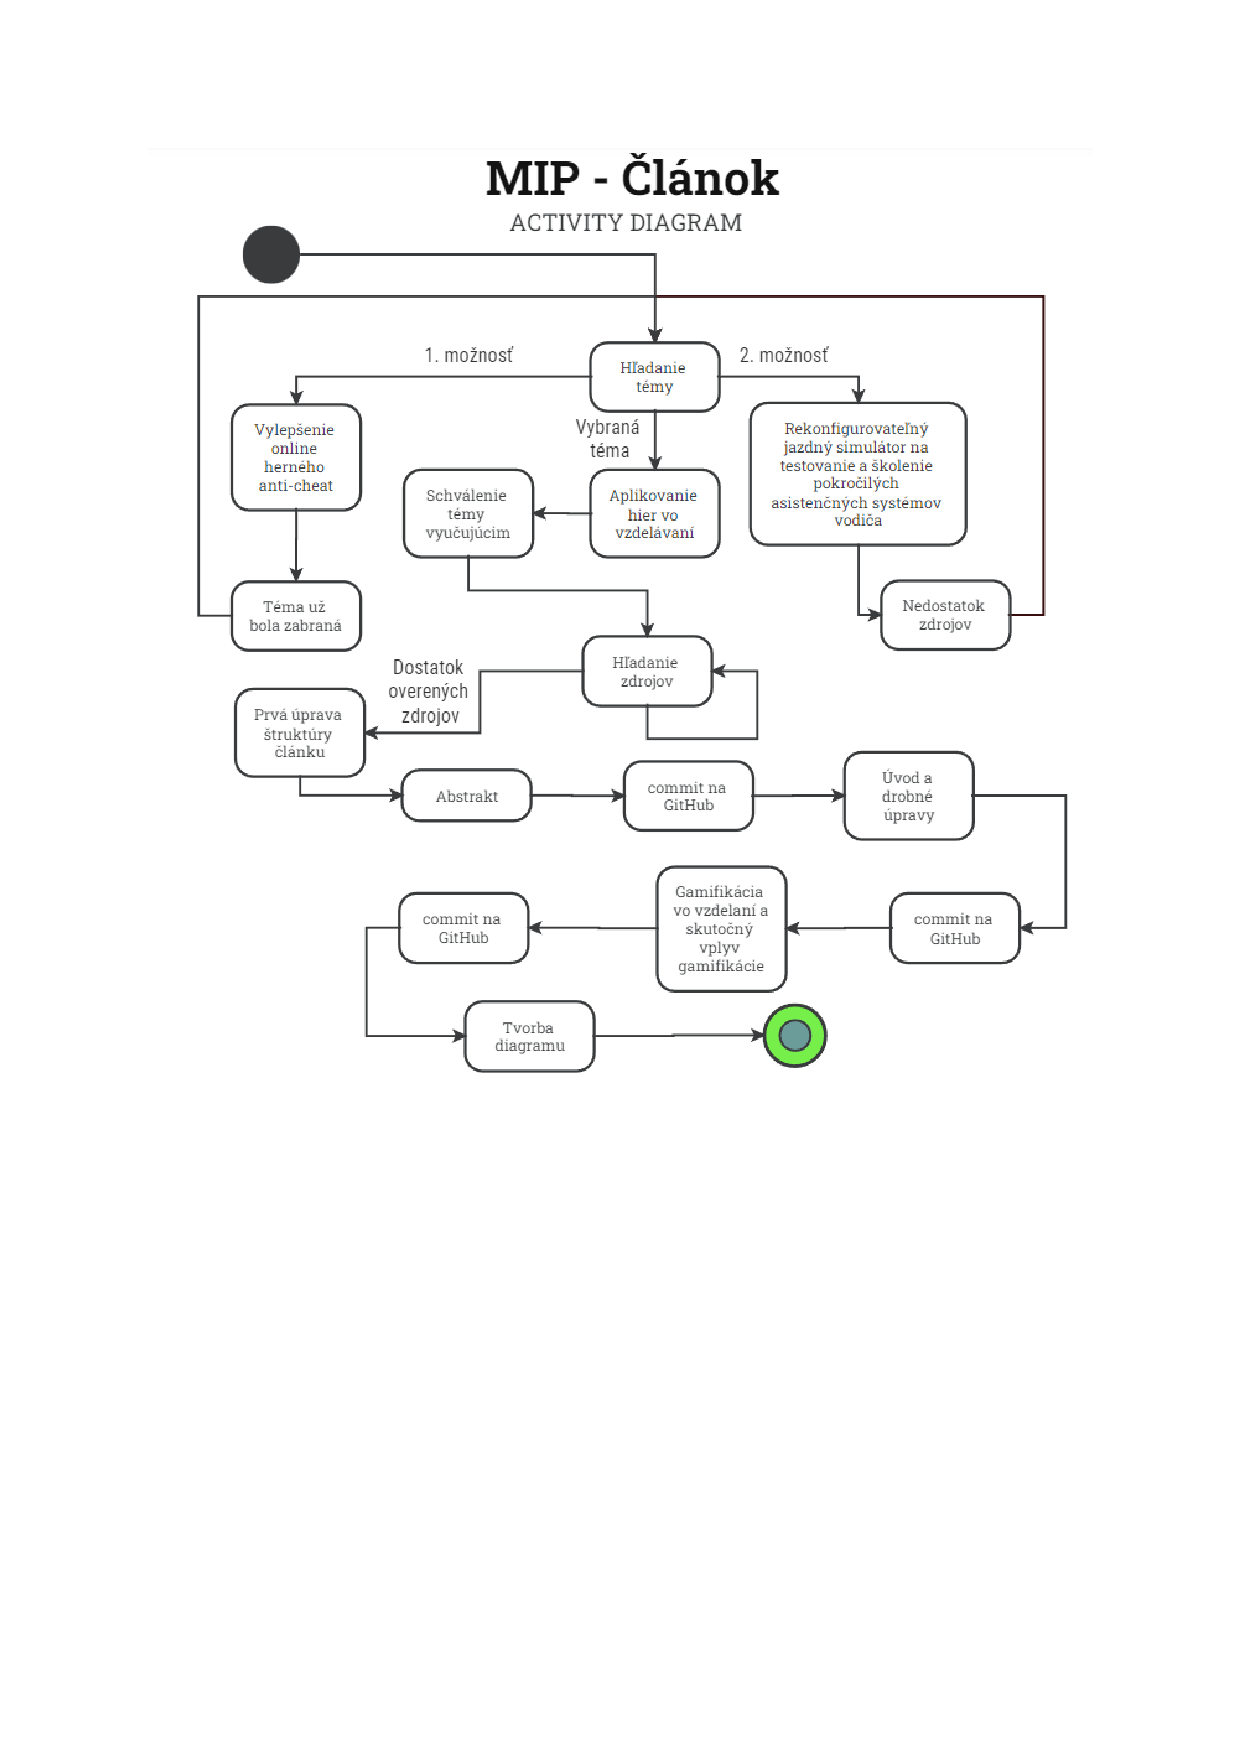
\includepdf[scale=0.8]{diagram.pdf} %k tomuto obrázku nemám zdrojový kód, pretože na stránke, kde som to robil sa obrázok nedal stiahnuť, preto som urobil iba screenshot, ale mam ho vo formáte pdf

\bibliography{literatura}
\bibliographystyle{abbrv} 
\end{document}
